\documentclass[a4paper, 12pt]{article}
\usepackage{geometry}
\geometry{a4paper,
total={170mm,257mm},left=2cm,right=2cm,
top=2cm,bottom=2cm}

\usepackage{mathtext}
\usepackage{amsmath}
\usepackage[utf8]{inputenc}
\usepackage[english,russian]{babel}
\usepackage{graphicx, float}
\usepackage{tabularx, colortbl}
\usepackage{caption}
\captionsetup{labelsep=period}

\newcommand{\parag}[1]{\paragraph*{#1:}}
\DeclareSymbolFont{T2Aletters}{T2A}{cmr}{m}{it}
\newcounter{Points}
\setcounter{Points}{1}
\newcommand{\point}{\arabic{Points}. \addtocounter{Points}{1}}
\newcolumntype{C}{>{\centering\arraybackslash}X}

\author{Калинин Даниил, Б01-110}
\date{\today}
\title{Лабораторная работа 1.2.1\\Определение скорости полета пули при помощи баллистического маятника}

\begin{document}
\maketitle

\parag {Цель работы}
определить скорость полета пули, применяя законы
сохранения и используя баллистические маятники.
   
\parag {В работе используются}
духовое ружье на штативе, осветлитель, оптическая система для измерения отклонений маятника, измерительная линейка, пули и весы для их вовешивания, а также 6аллистические маятники.

\parag {Теоритическая справка} ~\\
В первой части работы используется баллистический маятник, совершающий поступательное движение. Чертеж установки изображен на рисунке \ref{pic:pend1}.

\begin{figure}[H]
    \centering
    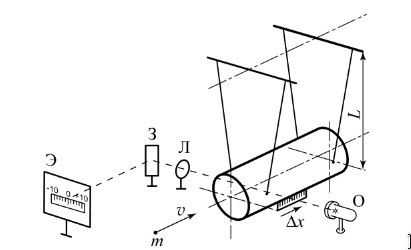
\includegraphics[width=0.8\linewidth]{pendulum1.png}
    \caption{Схема установки первой части работы.}
    \label{pic:pend1}
\end{figure}

Пусть масса маятника равна $M$, масса пули -- $m$, скорость пули перед ударом -- $u$, а скорость цилиндра установки после неупругого соударения: $V$. тогда по закону сохранения импульса имеем:

\begin{equation}
    mu = \left(M + m\right) V    
\end{equation}

Учитывая, что масса маятника много больше массы пули, получаем:

\begin{equation}
    u = \frac{M}{m}V
\end{equation}

По закону сохранения энергии, после попадания в него пули, маятник поднимется на высоту $h$, которая связана со скоростью цилиндра следующим образом:

\begin{equation}
    V^2 = 2gh
\end{equation}

Обозначим угол отклонения маятника за $\varphi$, длину нитей маятника за $L$, тогда:

\begin{align}
    h = L \left(1 - \cos\varphi\right) = 2L\sin^2\frac{\varphi}{2}, & \text{~~~где~~} \varphi \approx \frac{\Delta x}{L}
\end{align}

Используя вышеперечисленные формулы, получаем

\begin{equation}
    u = \frac{M}{m}\sqrt{\frac{g}{L}}\Delta x
    \label{eq:speed_for_1}
\end{equation}


Во второй части лабораторной работы используется крутильный баллистический маятник. Чертеж установки второй части работы приведен на рисунке \ref{pic:pend2}

\begin{figure}[H]
    \centering
    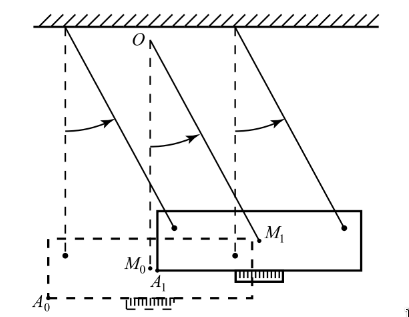
\includegraphics[width=0.8\linewidth]{pendulum2.png}
    \caption{Схема установки первой части работы.}
    \label{pic:pend2}
\end{figure}

Для определения скорости пули в этом случае, воспользуемся законом сохранения момента импульса в виде 

\begin{equation}
    mur = I\Omega  
\end{equation}

Здесь $r$ -- расстояние от линии пролета до оси вращения маятника, $I$ -- момент инерции маятника, $\Omega$ -- угловая скорость вращения маятника.

Запишем закон сохранения энергии:

\begin{equation}
    k \frac{\varphi^2}{2} = I\frac{\Omega^2}{2}  
\end{equation}

Где $k$ -- модуль кручения проволоки, а $\varphi$ -- максимальный угол поворота маятника.

Из вышеперечисленных формул получаем

\begin{equation}
    u = \varphi \frac{\sqrt{kI}}{mr}
    \label{eq:speed_for_2}
\end{equation}

Из рисунка \ref{pic:pend2} следует, что 

\begin{equation}
    \varphi \approx \frac{x}{2d}
    \label{eq:phi}
\end{equation}
Где $d$ -- расстояние от шкалы, до оси вращения маятника.

Произведение $kI$ можно определить, измерив периоды колебаний маятника с грузами $M$ и без них. Тогда периоды таких колебаний равны, соотвественно:

\begin{eqnarray}
    T_1 = 2\pi\sqrt{\dfrac{I}{k}} & T_2 = 2\pi\sqrt{\dfrac{I - 2MR^2}{k}}
\end{eqnarray}

Из этого получаем:

\begin{equation}
    \sqrt{kI} = \frac{4\pi M R^2 T_1}{T_1^2 - T_2^2}
    \label{eq:kI}
\end{equation}


Где $R$ -- расстояние от центров масс грузов $M$ до проволоки.


\parag {Ход работы} ~\\

\point Запишем погрешности измерительных приборов в таблицу \ref{tabl:inaccs}.

\begin{table}[H]
    \centering
    \begin{tabular}{|l|l|}
    \hline 
    Прибор                      & Погрешность                   \\ \hline
    Линейка                     & $\sigma = 0.5 $ мм.           \\ \hline
    Весы                        & $\sigma = 5 \cdot 10^{-4}$ гр.\\ \hline
    Шкала на первой установке   & $\sigma = 0.125$ мм.          \\ \hline
    Шкала на второй установке   & $\sigma = 0.5$ мм.            \\ \hline
    \end{tabular}
	\caption{Погрешности}
    \label{tabl:inaccs}
\end{table}


\point Измерим массы пулек, результаты занесем в таблицу \ref{tabl:masses_1}

\begin{table}[!h]
    \centering
    \begin{tabular}{|c|c|c|c|c|c|c|c|c|}
        \hline
        Номер пули      & 1 & 2 & 3 & 4 & 5  & 6 & 7 & 8 \\ \hline
        Масса пули, гр. & 0.509 & 0.512 & 0.511 & 0.5 & 0.51 & 0.5 & 0.5 & 0.501 \\ \hline
    \end{tabular}
    \caption{Результаты измерения масс пулек}
    \label{tabl:masses_1}
\end{table}

\point Измерим длину нитей, на которых подвешен маятник. Получим $L = 220 \pm 0.05$ см.

\point Измерим массу маятника. Получим $M = 2925 \pm 5$ гр.

\point Произведем серию экспериментов по выстрелу из духового ружья. Запишем отклонение маятника, а также расчитанную по формуле \ref{eq:speed_for_1} скорость для каждой пули в таблицу \ref{tabl:results_1}

\begin{table}[!h]
    \centering
    \begin{tabular}{|c|c|c|}
        \hline
        Номер пули & Отклонение маятника, мм. & Расчитанная скорость пули, м/с. \\ \hline
        1 &	11.25	& $136.5 \pm 4$  \\ \hline
        2 &	11.5	& $138.7 \pm 4$  \\ \hline
        3 &	11.5	& $139.0 \pm 4$  \\ \hline
        4 &	11.0	& $135.9 \pm 4$  \\ \hline
        5 &	11.25	& $136.2 \pm 4$  \\ \hline
        6 &	11.0	& $135.8 \pm 4$  \\ \hline
        7 &	11.0	& $135.8 \pm 4$  \\ \hline
        8 &	11.0	& $135.6 \pm 4$  \\ \hline

    \end{tabular}
    \caption{Результаты измерения отклонений маятника и значения скоростей пуль}
    \label{tabl:results_1}
\end{table}

\point Усредняя полученные значения скорости: $\bar{u} = 138.3 \pm 4$ м/с.

\point Перейдем ко второй установке. Измерим ее параметры, пользуясь обозначениями из теоретической части работы. Получим $r = 21$ см., $d = 57$ см., $R = 33$ см.

\point Теперь измерим периоды колебаний маятника без грузов и с ними. Результаты занесем в таблицу \ref{tabl:periods}.

\begin{table}
    \centering
    \begin{tabular}{|c|c|c|c|c|c|}
        \hline
        С грузами, $10 \cdot T_1$, с & 240 & 240 & 238 & 239 & 239 \\ \hline
        Без грузов, $10 \cdot T_2$, с & 180 & 179 & 178 & 180 & 182 \\ \hline
    \end{tabular}
    \caption{Результаты измерения периода колебаний маятника}
    \label{tabl:periods}
\end{table}

\point Пользуясь формулой \ref{eq:kI}, расчитаем величину $\sqrt{kI}$

\begin{equation*}
    \sqrt{kI} = (97 \pm 2)\cdot 10^{-2} \frac{кг \cdot м^2}{с}
\end{equation*}

\point Измерим и запишем в таблицу \ref{tabl:masses_2} массы второго набора пуль.

\begin{table}[!h]
    \centering
    \begin{tabular}{|c|c|c|c|c|c|c|c|c|}
        \hline
        Номер пули      & 1 & 2 & 3 & 4 & 5  & 6 & 7 & 8 \\ \hline
        Масса пули, гр. & 0.502 & 0.51 & 0.51 & 0.511 & 0.504 & 0.513 & 0.503 & 0.508 \\ \hline
    \end{tabular}
    \caption{Результаты измерения масс пулек}
    \label{tabl:masses_2}
\end{table}

\point Проведем серию экспериментов со второй установкой. Измерим отклонения маятника, а также по форумлам \ref{eq:phi} и \ref{eq:speed_for_2} расчитаем величины $\varphi$ и $u$. Результаты занесем в таблицу \ref{tabl:results_2}

\begin{table}[!h]
    \centering
    \begin{tabular}{|c|c|c|c|}
        \hline
        Номер пули & Отклонение маятника, см. & Угол поворота маятника, рад. & Расчитанная скорость пули, м/с. \\ \hline
        1 &	17.5	&	0.15	&	$141.25 \pm 2$ \\ \hline
        2 &	18.0	&	0.16	&	$143.00 \pm 2$ \\ \hline
        3 &	18.0	&	0.16	&	$143.00 \pm 2$ \\ \hline
        4 &	18.0	&	0.16	&	$142.72 \pm 2$ \\ \hline
        5 &	17.5	&	0.15	&	$140.69 \pm 2$ \\ \hline
        6 &	18.0	&	0.16	&	$142.17 \pm 2$ \\ \hline
        7 &	17.4	&	0.15	&	$140.16 \pm 2$ \\ \hline
        8 &	17.5	&	0.15	&	$139.58 \pm 2$ \\ \hline

    \end{tabular}
    \caption{Результаты измерения отклонений маятника и значения скоростей пуль}
    \label{tabl:results_2}
\end{table}

\point Усредняя значения скоростей, получим: $\bar{u} = 141.5 \pm 2$ м/с.

\parag {Заключение} ~\\
В работе были получены значения скорости пуль, выпущенных из духового ружья двумя способами: при помощи поступательного и крутильного баллистических маятников. Результаты: $\bar{u} = 138.3 \pm 4$ м/с. и $\bar{u_2} = 141.5 \pm 2$ м/с. совпали с точностью до погрешности. 

\end{document}
